\section{Evaluation}

\subsection{Best GoP}
The previous section indicates that reduce the keyframe interval may cut down the frame dropping. And in this section, we evaluate the method: reducing keyframe interval.
\textbf{Implementation and experiment setup.}
We design control experiments, where we control the outbound throughput of broadcaster to a certain level, and introduces a 2-second interruption. We record the number of frame drop as metrics to evaluate these methods. The frame rate in this paper usually equals to 30.

\begin{figure}[htb]
\centering
\begin{subfigure}[b]{.8\columnwidth}
\centering
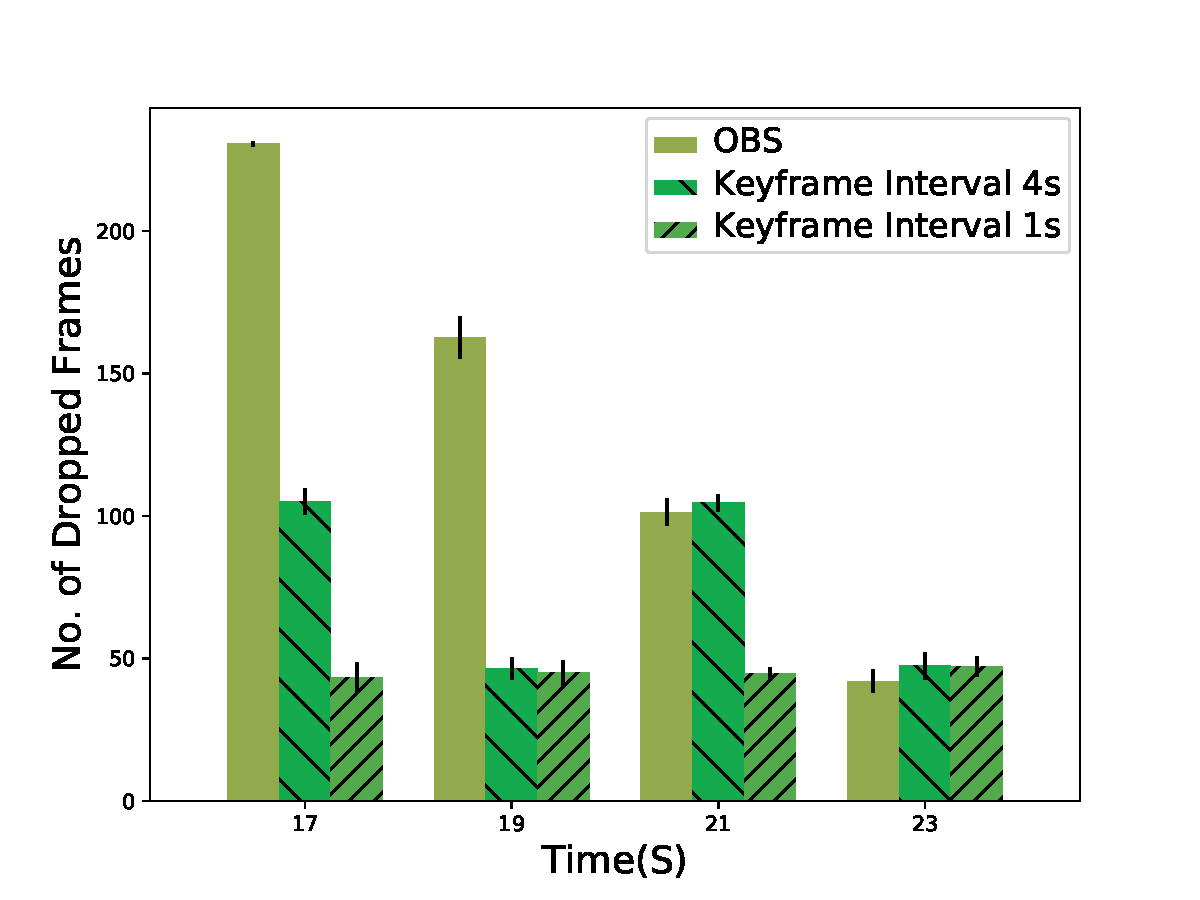
\includegraphics[width=\textwidth]{fig/eval_IframeInterval_drop.pdf}
\caption{Frame drop with varying I frame interval}
\label{fig:iframe-drop}\mylabel{fig:iframe-drop}
\end{subfigure}

\iffalse
\minipage{0.32\textwidth}
  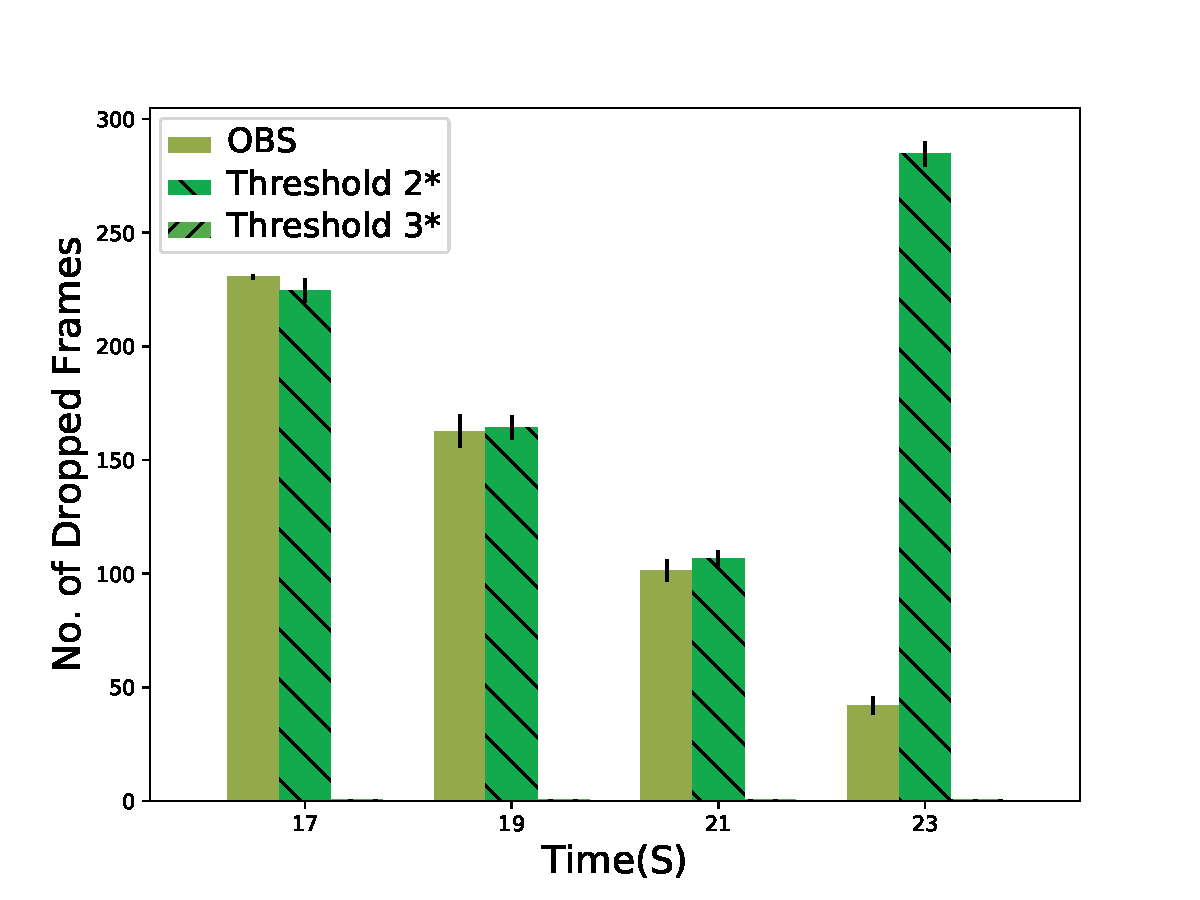
\includegraphics[width=\linewidth]{fig/eval_threshold_drop.pdf}
  \caption{Frame drop with varying threshold}
  \label{fig:threshold-drop}\mylabel{fig:threshold-drop}
\endminipage\hfill
\minipage{0.32\textwidth}
  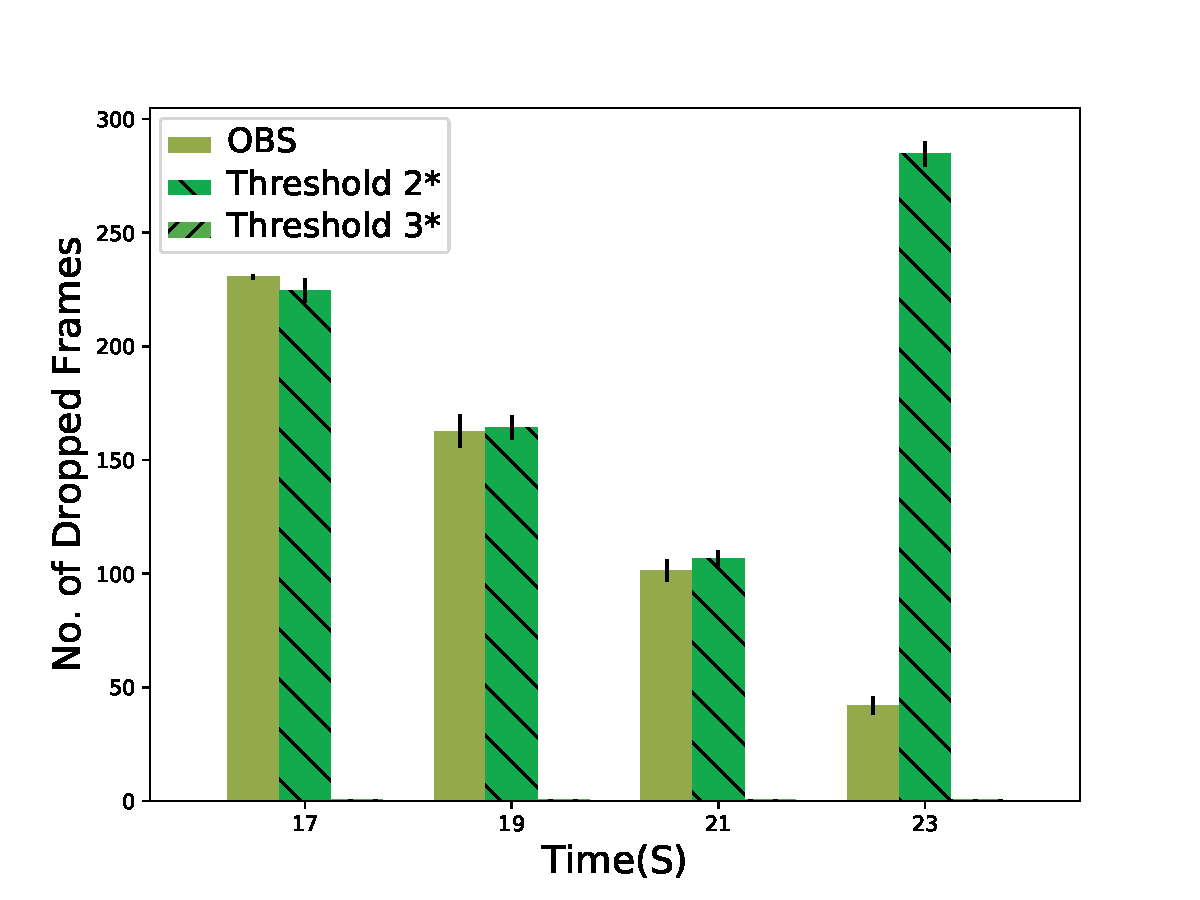
\includegraphics[width=\linewidth]{fig/eval_threshold_drop.pdf}
  \caption{Timeliness with varying I frame interval}
  \label{fig:iframe-timeliness}\mylabel{fig:iframe-timeliness}
\endminipage
\fi

\end{figure}

\iffalse
\begin{figure}
\centering
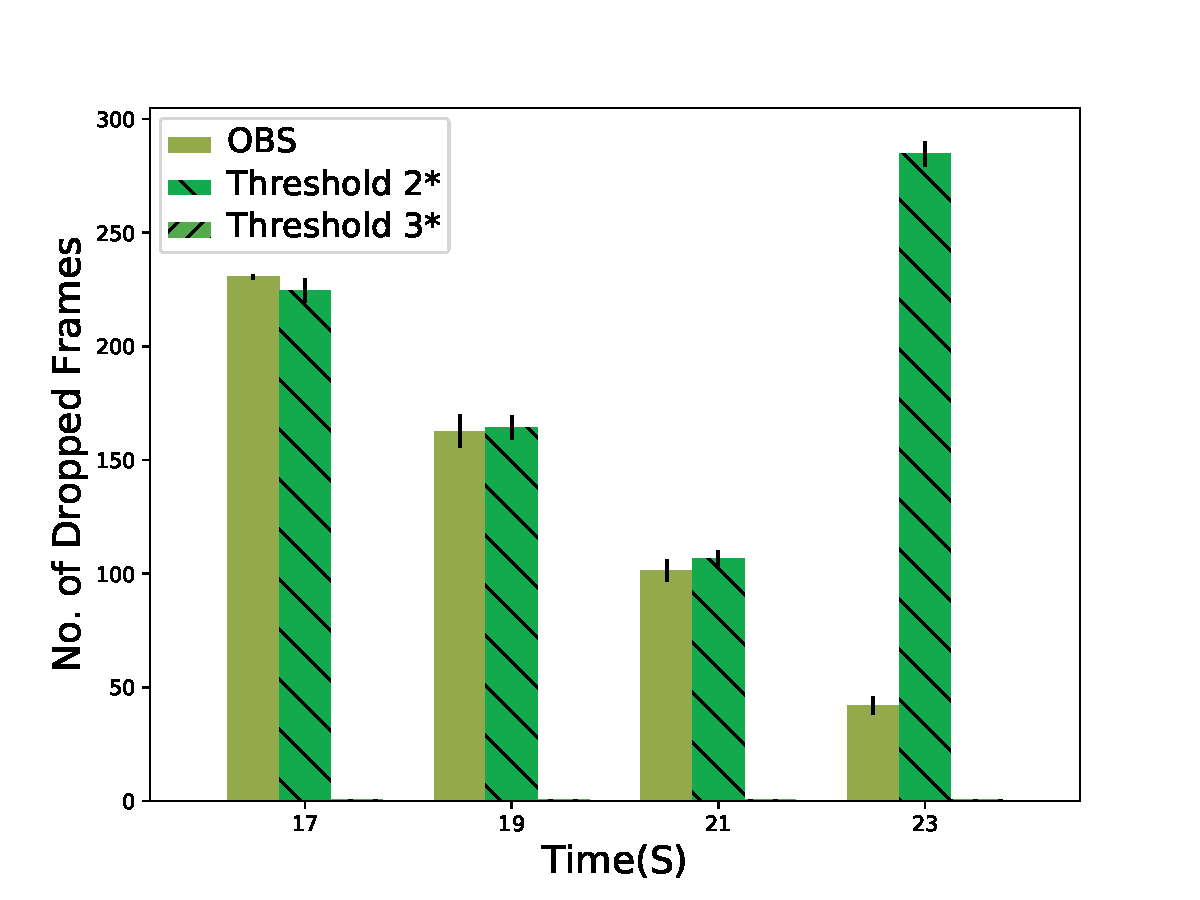
\includegraphics[width=0.32\textwidth]{fig/eval_threshold_drop.pdf}
\caption{Timeliness with varying threshold}
\label{fig:threshold-timeliness}\mylabel{fig:threshold-timeliness}
\end{figure}
\fi 
\textbf{Varying key frame interval.} The default I frame interval of OBS is 8 seconds, and we adjust it to be 4s and 2s in experiments. The frame drop are shown in Figure~\ref{fig:iframe-drop}. We can observe that in each individual experiment, when the interruption starts earlier in a GOP, more frames are dropped, because an early frame has more following frames depending on it. For example, for default setting, 8 second keyframe interval, when interruption starts at 17s, 19s, 21s, and 23s, the number of frame drop is 238, 164, 105, and 48.
Also, the number of frame drop appears to have the same period with the keyframe interval (e.g., when keyframe interval is 4s, the number of frame drop is 102, 47, 103, and 48 when interruption starts at 17s, 19s, 21s, and 23s, showing a period of 4s.).

Comparing bars within the group of 17s, we find that smaller keyframe interval significantly reduces the number of frame drop (i.e., from 238, to 102, and 46 when the interval is from 8s to 4s and 2s). However, this reduction is not significant for the group of 23s, because 23s is near the end of a GOP in all cases (8s, 4s, and 2s interval), there are only 1-second frames depending on the frame at 23s.

This experiment shows that if we can eliminate the dependency between frames, an occasional network jitter would only affect frames within a limited duration near the jitter, not cascadingly affecting frames in following several seconds. In practical use, reducing keyframe interval is an intractable issue because that adjust would cause video quality degradation. A tradeoff between video quality degradation and frame dropping needs to seriously solved.

\textbf{Video quality and GoP} As mentioned above, the value of GoP needs a tradeoff between video quality and frame dropping. To guide the choice of keyframe interval, we try to vary the GoP and encode many original streaming using x264 encoder \cite{x264}. A truth is that x264 encoder use the delta intermode coding, thus a larger GoP is much likely to introduce the accumulative errors, and GoP is suggested smaller than 250 frames. But how to determine the specific value is still intractable. We record SSIM as metrics. SSIM, the abbreviation of structural similarity, is a method for predicting quality of video, and is used for measuring the similarity of two images \cite{wang2004image}. The video dataset we use contains SD content, HD content, gaming, 4k content in variety \cite{video_dataset}. The relationship between normalized SSIM and gop size is displayed in Fig~\ref{fig:ssim_gop}.

We pick four from many videos to represent the result. From the figure, we can see when the GoP size is larger than 20, the SSIM keeps almost the same, with little changing.

Combined the previous two experiments, a GoP size larger than 20 can achieve better video quality; and a smaller gop size will reduce the frame dropping. We can see that value between $[20,60]$ may be almost the best choice for keyframe interval.

\iffalse
\begin{table}[htb]
\centering
\caption{No. of Dropped Frames}
\label{tab:bitrate}\mylabel{tab:bitrate}

\begin{tabular}{|l|l|l|l|l|}
\hline
Bitrate(kbps)          & 1000  & 1500  & 2000  & 2500  \\ \hline
Average Dropped Frames & 148.2 & 148.2 & 149.0 & 150.6 \\ \hline
\end{tabular}
\end{table}
\textbf{Varying bitrate.}
To make the conclusion more visible, we fix key frame interval to be 8s and introduce network interruption between 19s and 21s. In different experiments, we provide sufficient network bandwidth and vary the bitrate to be 1000kbps, 1500kbps, 2000kbps, and 2500kbps. The frame drop is shown in Table~\ref{tab:bitrate}. The different bitrates do not make much difference, the number of drop in all cases is about 149.

\textbf{Summary.} We summarize and get conclusions. First, reducing keyframe interval leads to less frame drop. Second, bitrate does not influence frame drop for the short-term case, but the quality of each picture. Preliminary Evaluation points out that a small GoP is one useful try.
\fi

\subsection{Greedy Drop Strategy}
To measure the performance, we compare the performance with two algorithms, there are respectively Oracle, OBS default. Oracle is the brute-force search to calculate the optimal solution, which has an exponential time complexity. We pick out one part from the dataset, and the trace lasts for $30$ seconds, and during the period both bandwidth fading and bandwidth fluctuating appears. The frame rate is $30$ fps, the total number of frame equals to $900$.

\begin{table}[tb]
\centering
\caption{The Reduction of Frame Drops Normalized to Default OBS}
\label{tab_drop}
{\setlength{\tabcolsep}{1pt}
\begin{tabular}{|c|c|l|}
\hline
\textbf{Algorithm} &\textbf{Play Failure(s)} & \textbf{Percentage}    \\ \hline
Oracle    &265    &$80\%$           \\ \hline
GreedyDrop  &274  &$85.6\%$              \\ \hline
\end{tabular}}
\vspace{-0.1in}
\end{table}

\begin{figure}[htb]
\centering
\begin{subfigure}[b]{.45\columnwidth}
\centering
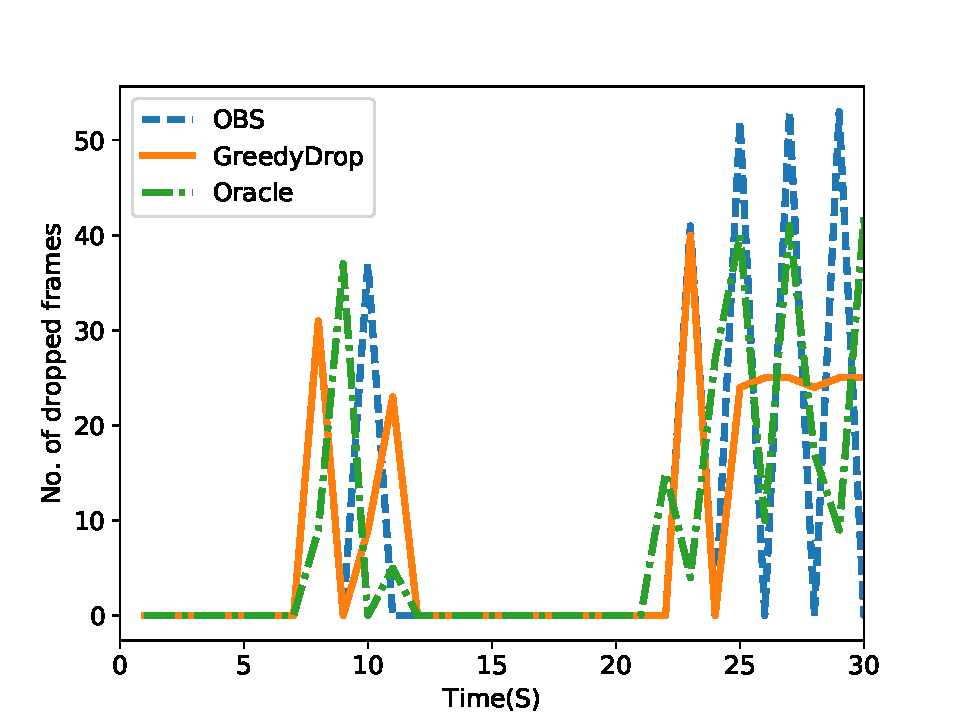
\includegraphics[width=\linewidth]{fig/drop-buffer.pdf}
\caption{No. of frame drop}
\label{fig:drop-buffer}\mylabel{fig:drop-buffer}
\end{subfigure}
\begin{subfigure}[b]{.45\columnwidth}
\centering
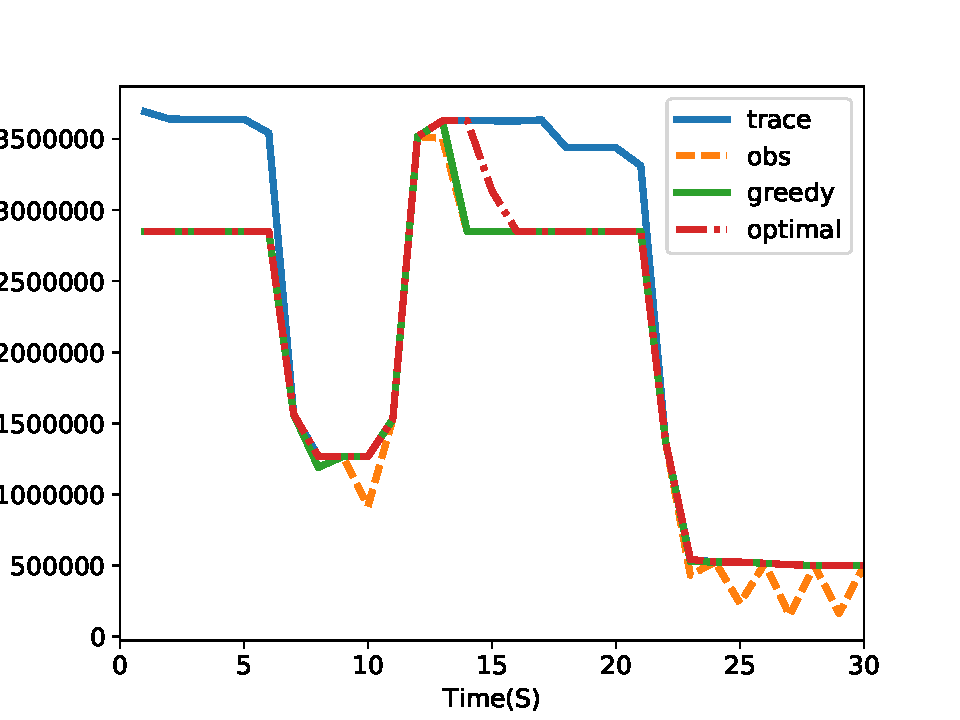
\includegraphics[width=\linewidth]{fig/drop-bandwidth.pdf}
\caption{Real-time throughput}
\label{fig:drop-bandwidth}\mylabel{fig:drop-bandwidth}
\end{subfigure}
\caption{Comparison of different frame drop strategy}
\vspace{-0.15in}
\end{figure} 
The number of dropped frames is displayed in the table~\ref{tab_drop}. OBS dropped the most frames among three, and GreedyDrop reduce $15\%$, which is a notable improvement. And the gap between GreedyDrop and Oracle is small, less than $5\%$. The real-time frame drop and throughput is showed in Figures~\ref{fig:drop-buffer}~\ref{fig:drop-bandwidth}. The main period of frame dropping locates in 5-10s and 20-30s. All three algorithms preform similar in 5-10s, but optimal will save more frames before the network recovers, and keep a high bandwidth at 10-15s. The frame drop of OBS waves at a high variance in 20-30s, but GreedyDrop almost keep the same value. Because GreedyDrop only drops the undecodable frames of the first GoP. For each GoP, the begin is send to receiver, and the rest ones is dropped, so for each time, the frame drop and the throughput keeps still. Optimal also shakes, but with a small variance. Considering both time complexity and performance, GreedyDrop is a good choice.


\subsection{Greedy Adaptive Bitrate}
\begin{figure*}[htb]
\minipage{0.32\textwidth}
  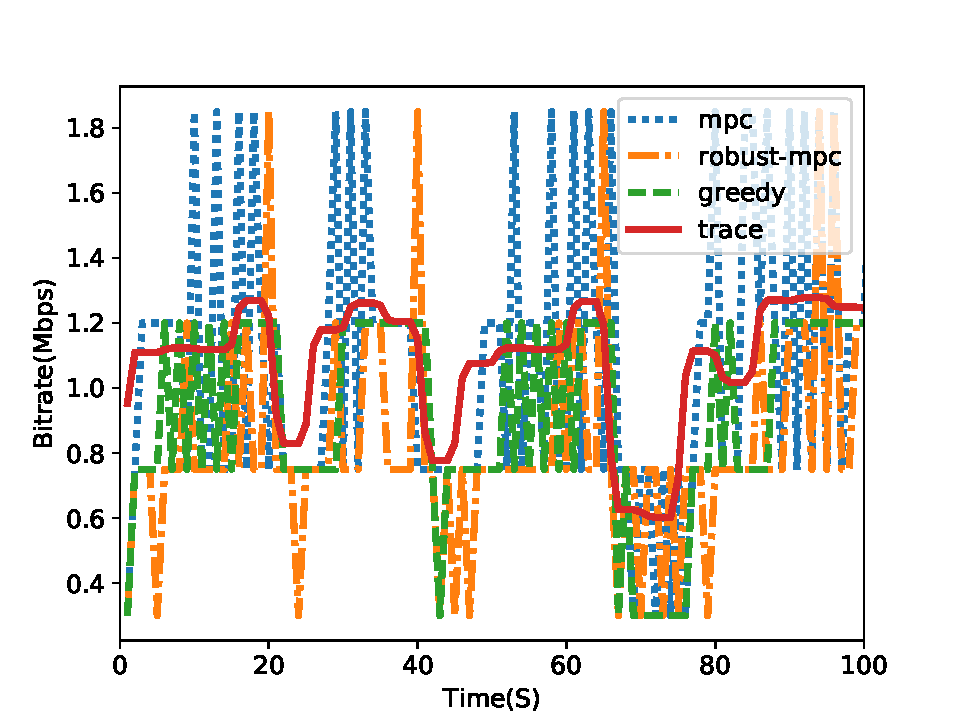
\includegraphics[width=\linewidth]{fig/specific_fcc.pdf}
  \caption{Throughput of FCC dataset}
  \vspace{-0.23in}
  \label{fig:fcc_specific}\mylabel{fig:fcc_specific}
\endminipage
\hfill
\minipage{0.32\textwidth}
  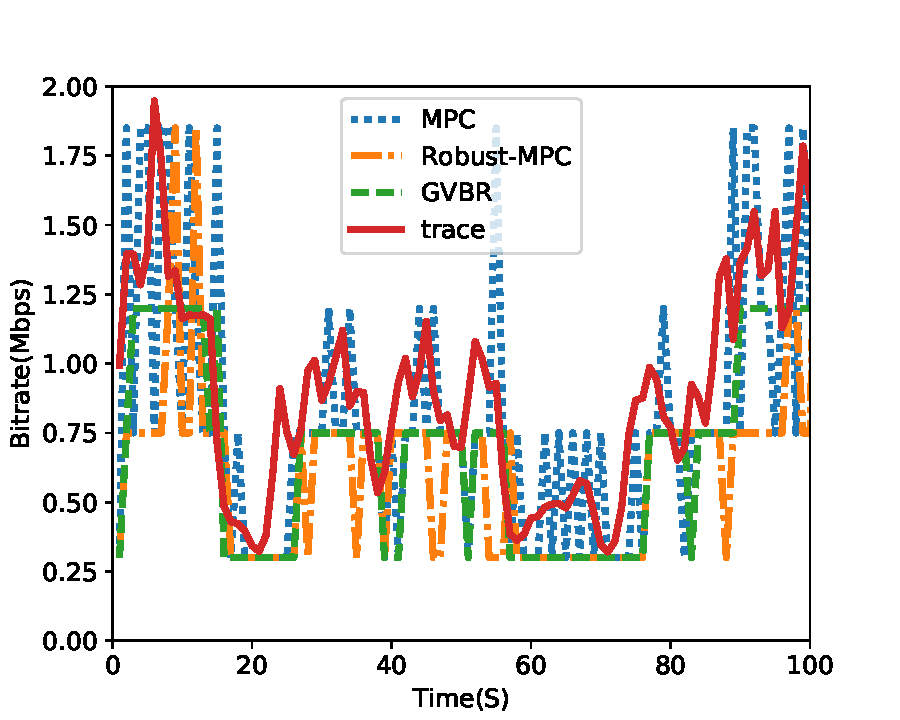
\includegraphics[width=\linewidth]{fig/specific_hsdpa.pdf}
  \caption{Throughput of HSDPA dataset}
  \vspace{-0.23in}
  \label{fig:specific_hsdpa}\mylabel{fig:specific_hsdpa}
\endminipage
\hfill
\minipage{0.32\textwidth}
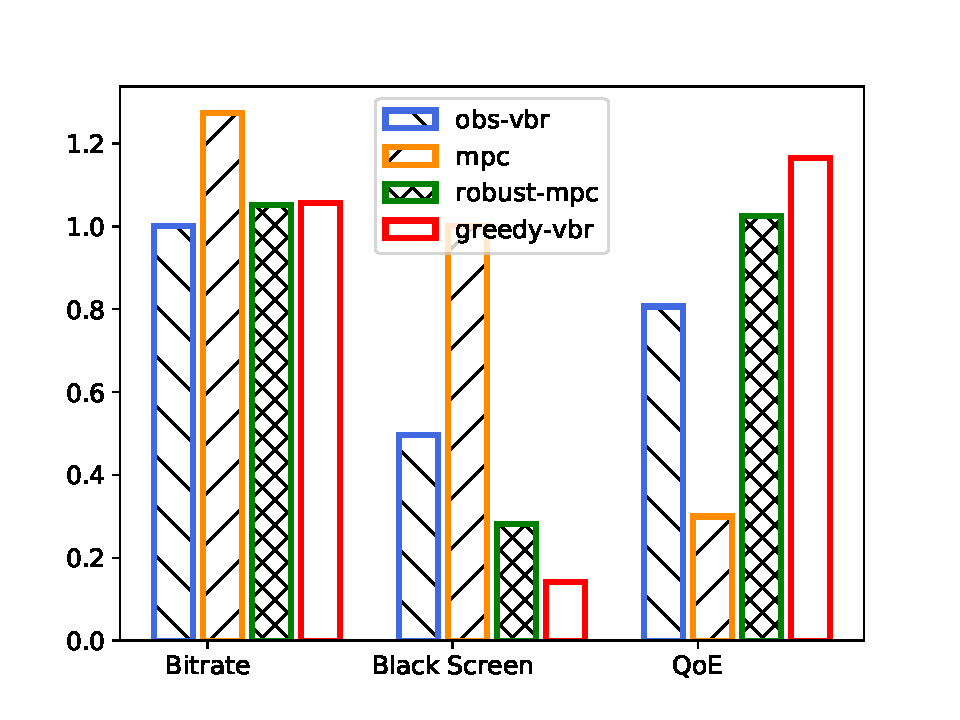
\includegraphics[width=\textwidth]{fig/massive_qoe.pdf}
\caption{Normalized bitrate, play failure and QoE}
\vspace{-0.23in}
\label{fig:vbr-qoe}\mylabel{fig:vbr-qoe}
\endminipage
\end{figure*}

\begin{figure*}[htb]
\minipage{0.32\textwidth}
  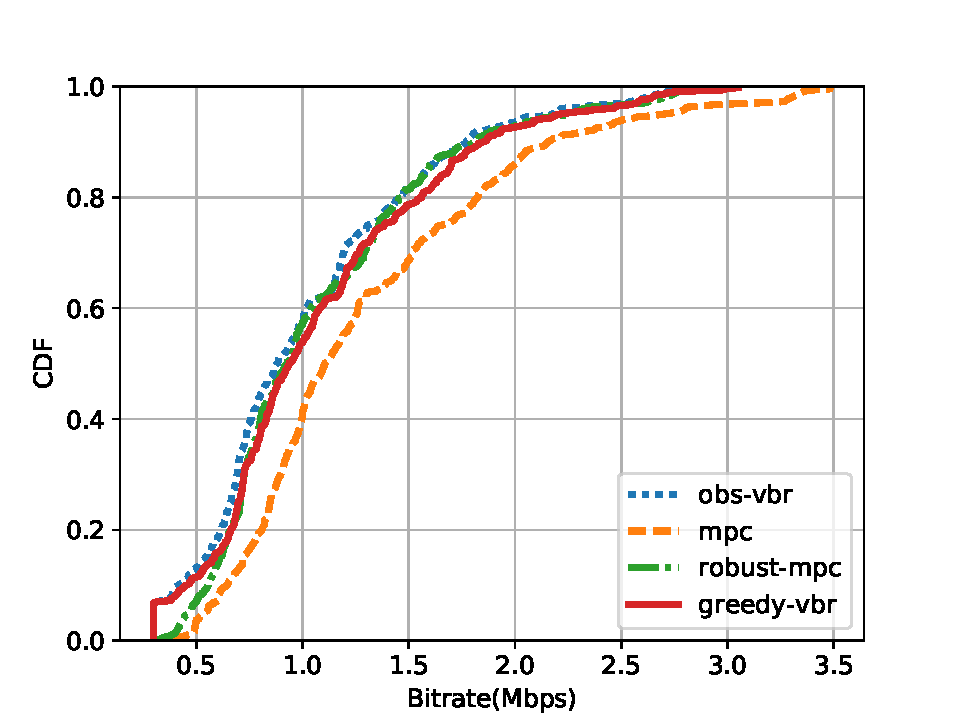
\includegraphics[width=\linewidth]{fig/massive-bitrate-cdf.pdf}
  \caption{CDF of Bitrate}
  \vspace{-0.25in}
  \label{fig:vbr-bitrate-cdf}\mylabel{fig:vbr-bitrate-cdf}
\endminipage
\minipage{0.32\textwidth}
  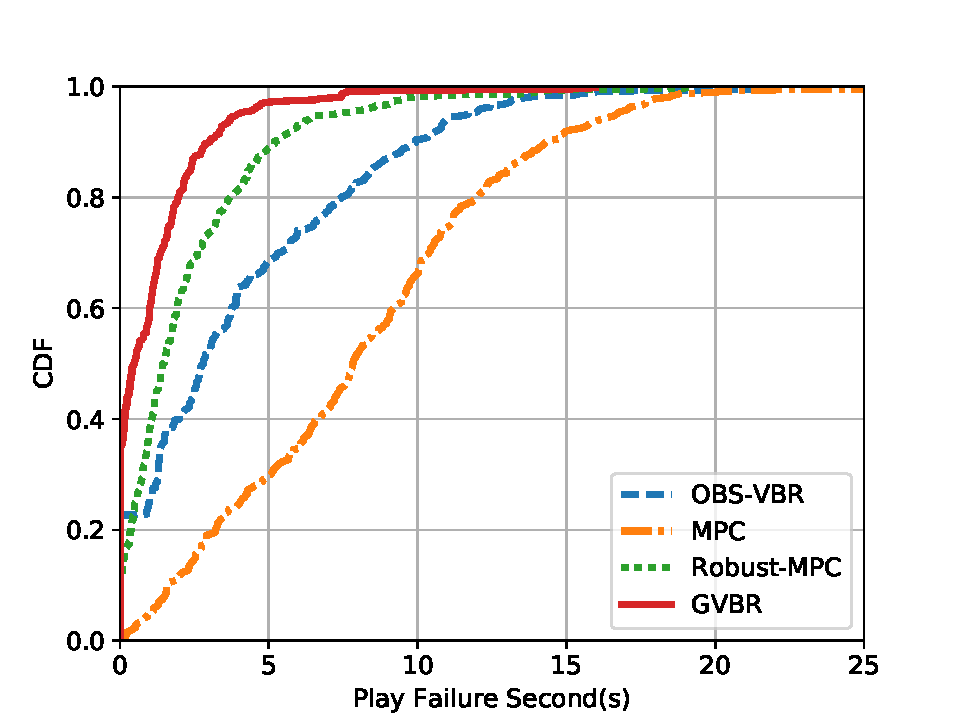
\includegraphics[width=\linewidth]{fig/massive-drop-cdf.pdf}
  \caption{CDF of Play Failure Seconds}
  \vspace{-0.25in}
  \label{fig:vbr-drop-cdf}\mylabel{fig:vbr-drop-cdf}
\endminipage
\minipage{0.32\textwidth}
  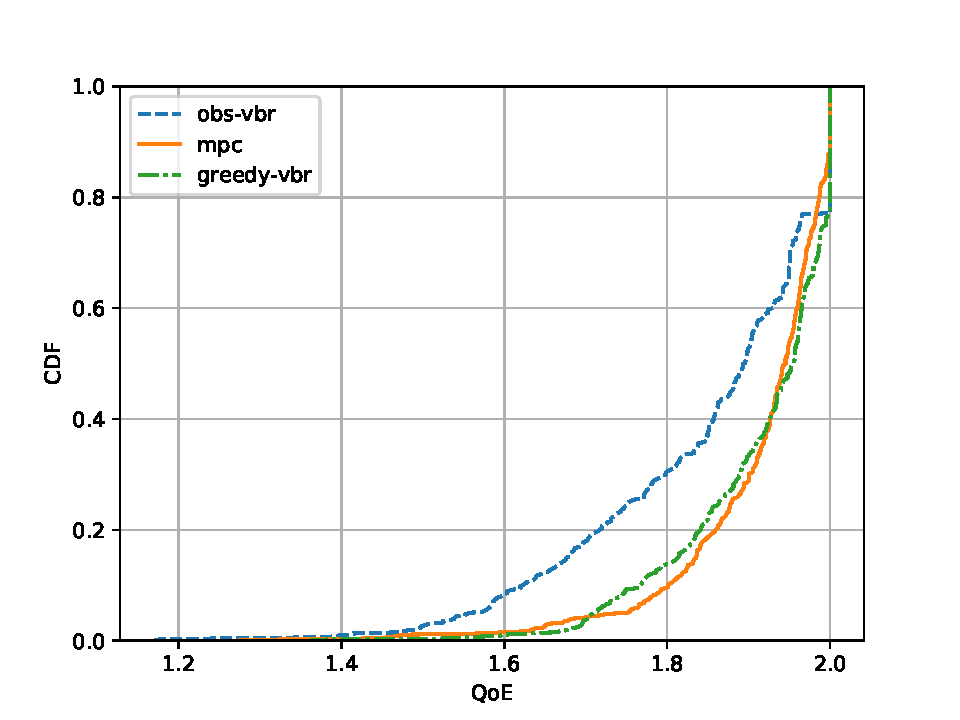
\includegraphics[width=\linewidth]{fig/massive-qoe-cdf.pdf}
  \caption{CDF of Normalized QoE }
  \vspace{-0.25in}
  \label{fig:vbr-qoe-cdf}\mylabel{fig:vbr-qoe-cdf}
\endminipage
\end{figure*} 
We compared GVBR algorihtm towards three algorithms which work excellently in VOD bitrate adaptation:
\begin{itemize}
  \item OBS: A simple video adaptation method, each time choose the bitrate exactly lower than the estimated bandwidth. Besides, the default drop strategy in obs. Harmonic mean is used for bandwidth estimation.
  \item MPC: use buffer state(number and size of frames, and type of frames, I/P/B) and bandwidth predictions to calculate the optimal bitrate operation in future several time slots; and use the first bitrate choice in next time slot.
  \item Robust-MPC: use the approach similar with MPC, and correct the estimated bandwidth by considering the prediction error in past several time slots. New estimated bandwidth equals to the original estimated bandwidth divide the prediction error.
\end{itemize}
Robust-MPC is the state-of-art video adaptation algorithm. The MPC theory can also be applied in live streaming scenario.
Detailed comparison results are shown in Figures ~\ref{fig:fcc_specific} and \ref{fig:specific_hsdpa}. In these two figures, the red real line is one real-world trace. Without predication error, MPC prefers to choose more higher bitrate than Robust-MPC. Besides, these two MPC algorihtm always shake around the real bandwidth. In both cases, the MPC and Roubust-MPC switch more bitrate than GVBR. Because GVBR tends to choose the lower bitrate than the throughput, and when comes the small bandwidth fluctuation, GVBR is less likely to shake. But MPC struggles to achieve the optimal utility, and when the bandwidth increases a little, MPC has the potential to choose a higher bitrate to maximize the first item in \ref{vbr-formulation}.

A massive simulation is displayed in Figure \ref{fig:vbr-qoe}. We use the combined dataset, FCC and HSDPA to evaluate GVBR algorithm. Normalized qoe is calculated in the figure. Among all, MPC has the max bitrate qoe, because the bandwidth estimation is aggressive and MPC has the potential to choose higher bitrate. Three others reach almost the same average bitrate, with little difference, but GVBR is a little higher. With higher bitrate, MPC also drops the most frames, and the time of play failure is longest. GVBR reduces the play failure to a small value, 50\% reduction compared with Robust-MPC. With higher bitrate and lower play failure, GVBR definitely preforms the best, with the highest QoE.

Cdf figures about each metric is as follows, \ref{fig:vbr-bitrate-cdf}, \ref{fig:vbr-drop-cdf}, \ref{fig:vbr-qoe-cdf}. In \ref{fig:vbr-bitrate-cdf}, GVBR lies in the right of Robust-MPC and OBS, with a higher bitrate. $98\%$ of the paly failure is less than 5s in GVBR, about 40\% play fluently with no failure. Only 2\% of GVBR receive poor qoe, the rest 98\% has a high qoe lies in [0.8,1].

The total frame dropping compared with original OBS is reduced by 96\%. The play failure time of original OBS method with constant bitrate is 26s in average, and GVBR has a 1s play failure time.

As all, GVBR achieve a higher bitrate, and at the same time reduce the play failure to little.

